\documentclass[1p]{elsarticle_modified}
%\bibliographystyle{elsarticle-num}

%\usepackage[colorlinks]{hyperref}
%\usepackage{abbrmath_seonhwa} %\Abb, \Ascr, \Acal ,\Abf, \Afrak
\usepackage{amsfonts}
\usepackage{amssymb}
\usepackage{amsmath}
\usepackage{amsthm}
\usepackage{scalefnt}
\usepackage{amsbsy}
\usepackage{kotex}
\usepackage{caption}
\usepackage{subfig}
\usepackage{color}
\usepackage{graphicx}
\usepackage{xcolor} %% white, black, red, green, blue, cyan, magenta, yellow
\usepackage{float}
\usepackage{setspace}
\usepackage{hyperref}

\usepackage{tikz}
\usetikzlibrary{arrows}

\usepackage{multirow}
\usepackage{array} % fixed length table
\usepackage{hhline}

%%%%%%%%%%%%%%%%%%%%%
\makeatletter
\renewcommand*\env@matrix[1][\arraystretch]{%
	\edef\arraystretch{#1}%
	\hskip -\arraycolsep
	\let\@ifnextchar\new@ifnextchar
	\array{*\c@MaxMatrixCols c}}
\makeatother %https://tex.stackexchange.com/questions/14071/how-can-i-increase-the-line-spacing-in-a-matrix
%%%%%%%%%%%%%%%

\usepackage[normalem]{ulem}

\newcommand{\msout}[1]{\ifmmode\text{\sout{\ensuremath{#1}}}\else\sout{#1}\fi}
%SOURCE: \msout is \stkout macro in https://tex.stackexchange.com/questions/20609/strikeout-in-math-mode

\newcommand{\cancel}[1]{
	\ifmmode
	{\color{red}\msout{#1}}
	\else
	{\color{red}\sout{#1}}
	\fi
}

\newcommand{\add}[1]{
	{\color{blue}\uwave{#1}}
}

\newcommand{\replace}[2]{
	\ifmmode
	{\color{red}\msout{#1}}{\color{blue}\uwave{#2}}
	\else
	{\color{red}\sout{#1}}{\color{blue}\uwave{#2}}
	\fi
}

\newcommand{\Sol}{\mathcal{S}} %segment
\newcommand{\D}{D} %diagram
\newcommand{\A}{\mathcal{A}} %arc


%%%%%%%%%%%%%%%%%%%%%%%%%%%%%5 test

\def\sl{\operatorname{\textup{SL}}(2,\Cbb)}
\def\psl{\operatorname{\textup{PSL}}(2,\Cbb)}
\def\quan{\mkern 1mu \triangleright \mkern 1mu}

\theoremstyle{definition}
\newtheorem{thm}{Theorem}[section]
\newtheorem{prop}[thm]{Proposition}
\newtheorem{lem}[thm]{Lemma}
\newtheorem{ques}[thm]{Question}
\newtheorem{cor}[thm]{Corollary}
\newtheorem{defn}[thm]{Definition}
\newtheorem{exam}[thm]{Example}
\newtheorem{rmk}[thm]{Remark}
\newtheorem{alg}[thm]{Algorithm}

\newcommand{\I}{\sqrt{-1}}
\begin{document}

%\begin{frontmatter}
%
%\title{Boundary parabolic representations of knots up to 8 crossings}
%
%%% Group authors per affiliation:
%\author{Yunhi Cho} 
%\address{Department of Mathematics, University of Seoul, Seoul, Korea}
%\ead{yhcho@uos.ac.kr}
%
%
%\author{Seonhwa Kim} %\fnref{s_kim}}
%\address{Center for Geometry and Physics, Institute for Basic Science, Pohang, 37673, Korea}
%\ead{ryeona17@ibs.re.kr}
%
%\author{Hyuk Kim}
%\address{Department of Mathematical Sciences, Seoul National University, Seoul 08826, Korea}
%\ead{hyukkim@snu.ac.kr}
%
%\author{Seokbeom Yoon}
%\address{Department of Mathematical Sciences, Seoul National University, Seoul, 08826,  Korea}
%\ead{sbyoon15@snu.ac.kr}
%
%\begin{abstract}
%We find all boundary parabolic representation of knots up to 8 crossings.
%
%\end{abstract}
%\begin{keyword}
%    \MSC[2010] 57M25 
%\end{keyword}
%
%\end{frontmatter}

%\linenumbers
%\tableofcontents
%
\newcommand\colored[1]{\textcolor{white}{\rule[-0.35ex]{0.8em}{1.4ex}}\kern-0.8em\color{red} #1}%
%\newcommand\colored[1]{\textcolor{white}{ #1}\kern-2.17ex	\textcolor{white}{ #1}\kern-1.81ex	\textcolor{white}{ #1}\kern-2.15ex\color{red}#1	}

{\Large $\underline{12a_{0506}~(K12a_{0506})}$}

\setlength{\tabcolsep}{10pt}
\renewcommand{\arraystretch}{1.6}
\vspace{1cm}\begin{tabular}{m{100pt}>{\centering\arraybackslash}m{274pt}}
\multirow{5}{120pt}{
	\centering
	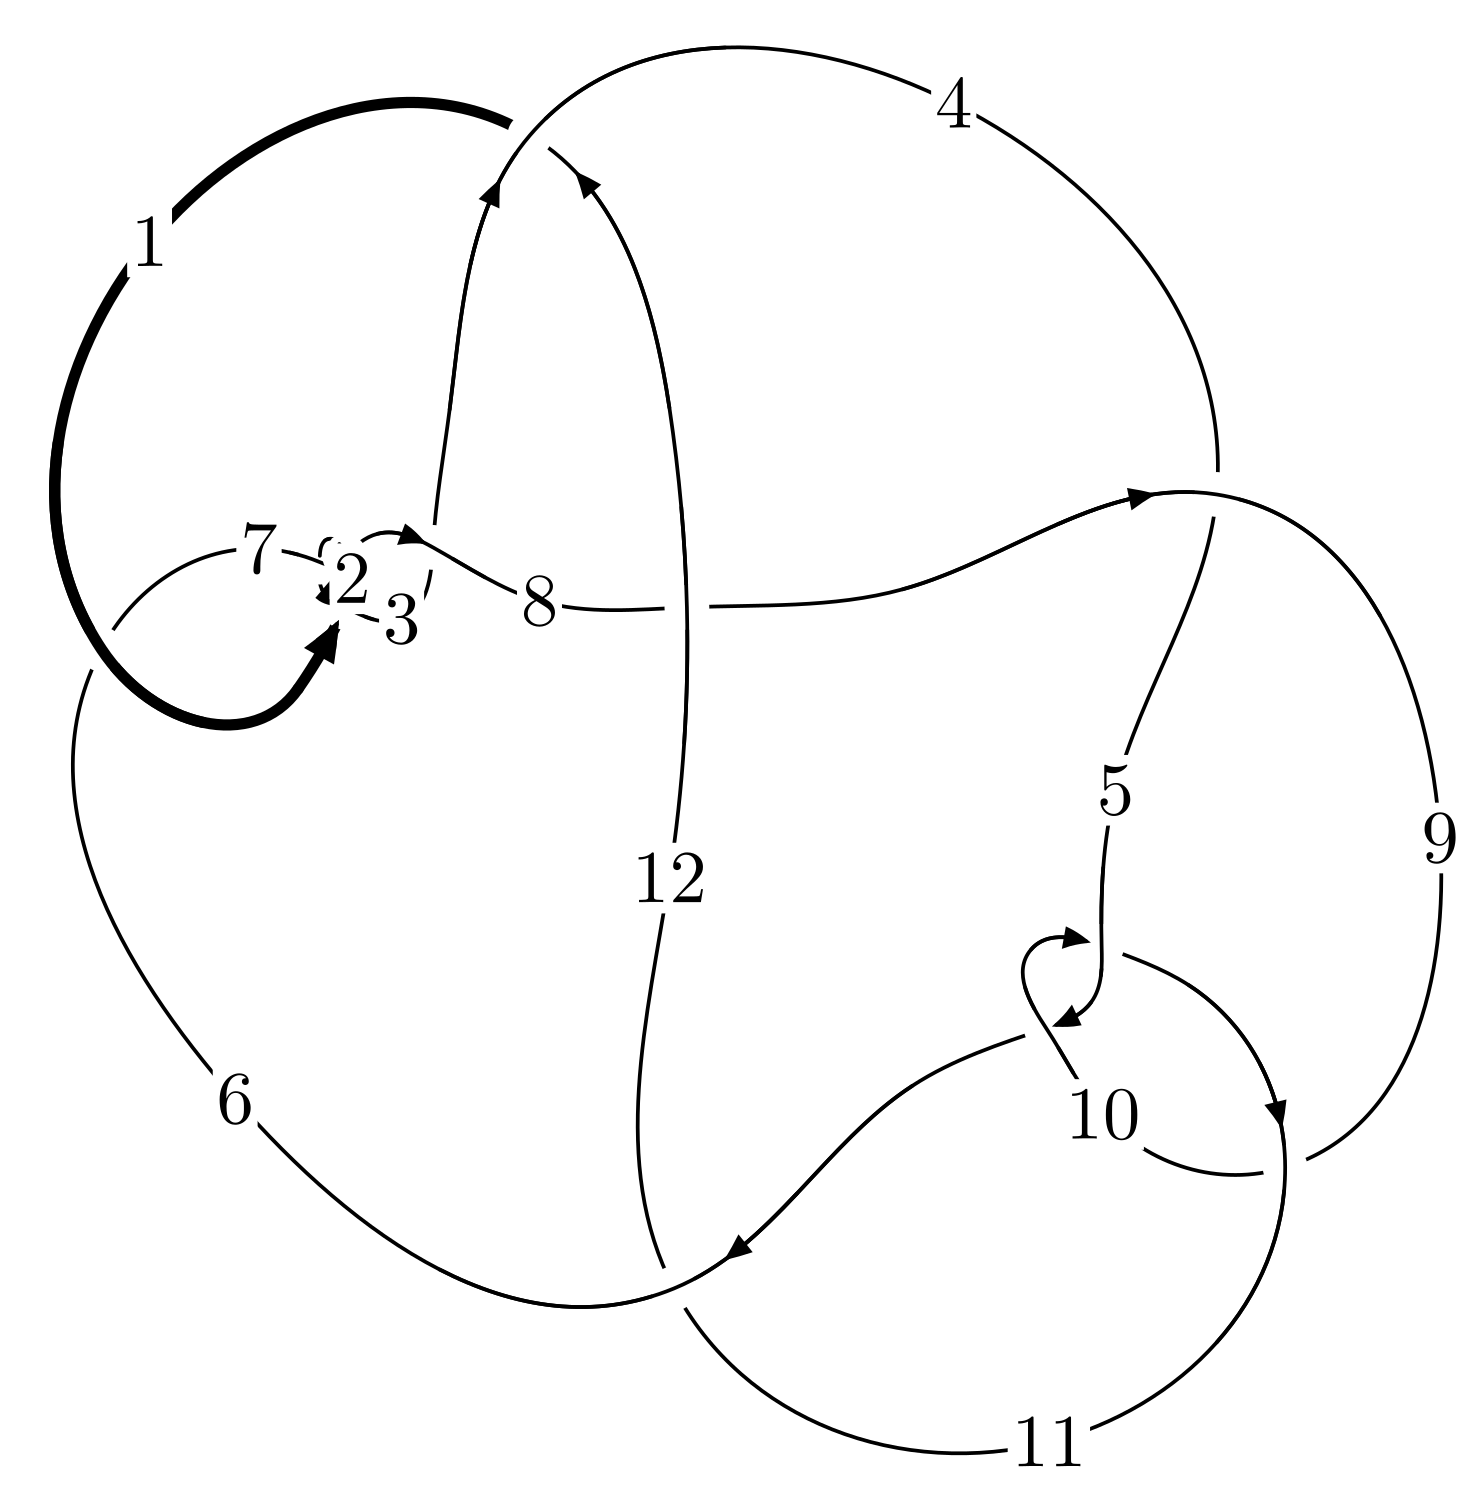
\includegraphics[width=112pt]{../../../GIT/diagram.site/Diagrams/png/1307_12a_0506.png}\\
\ \ \ A knot diagram\footnotemark}&
\allowdisplaybreaks
\textbf{Linearized knot diagam} \\
\cline{2-2}
 &
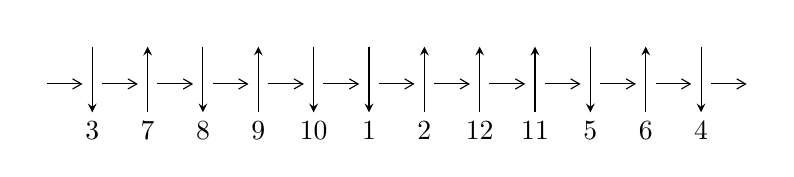
\begin{tikzpicture}[x=20pt, y=17pt]
	% nodes
	\node (C0) at (0, 0) {};
	\node (C1) at (1, 0) {};
	\node (C1U) at (1, +1) {};
	\node (C1D) at (1, -1) {3};

	\node (C2) at (2, 0) {};
	\node (C2U) at (2, +1) {};
	\node (C2D) at (2, -1) {7};

	\node (C3) at (3, 0) {};
	\node (C3U) at (3, +1) {};
	\node (C3D) at (3, -1) {8};

	\node (C4) at (4, 0) {};
	\node (C4U) at (4, +1) {};
	\node (C4D) at (4, -1) {9};

	\node (C5) at (5, 0) {};
	\node (C5U) at (5, +1) {};
	\node (C5D) at (5, -1) {10};

	\node (C6) at (6, 0) {};
	\node (C6U) at (6, +1) {};
	\node (C6D) at (6, -1) {1};

	\node (C7) at (7, 0) {};
	\node (C7U) at (7, +1) {};
	\node (C7D) at (7, -1) {2};

	\node (C8) at (8, 0) {};
	\node (C8U) at (8, +1) {};
	\node (C8D) at (8, -1) {12};

	\node (C9) at (9, 0) {};
	\node (C9U) at (9, +1) {};
	\node (C9D) at (9, -1) {11};

	\node (C10) at (10, 0) {};
	\node (C10U) at (10, +1) {};
	\node (C10D) at (10, -1) {5};

	\node (C11) at (11, 0) {};
	\node (C11U) at (11, +1) {};
	\node (C11D) at (11, -1) {6};

	\node (C12) at (12, 0) {};
	\node (C12U) at (12, +1) {};
	\node (C12D) at (12, -1) {4};
	\node (C13) at (13, 0) {};

	% arrows
	\draw[->,>={angle 60}]
	(C0) edge (C1) (C1) edge (C2) (C2) edge (C3) (C3) edge (C4) (C4) edge (C5) (C5) edge (C6) (C6) edge (C7) (C7) edge (C8) (C8) edge (C9) (C9) edge (C10) (C10) edge (C11) (C11) edge (C12) (C12) edge (C13) ;	\draw[->,>=stealth]
	(C1U) edge (C1D) (C2D) edge (C2U) (C3U) edge (C3D) (C4D) edge (C4U) (C5U) edge (C5D) (C6U) edge (C6D) (C7D) edge (C7U) (C8D) edge (C8U) (C9D) edge (C9U) (C10U) edge (C10D) (C11D) edge (C11U) (C12U) edge (C12D) ;
	\end{tikzpicture} \\
\hhline{~~} \\& 
\textbf{Solving Sequence} \\ \cline{2-2} 
 &
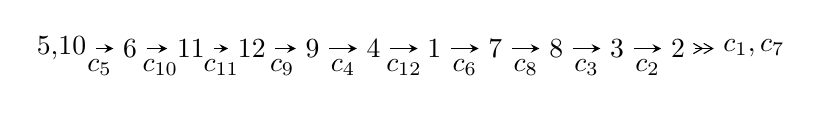
\begin{tikzpicture}[x=22pt, y=7pt]
	% node
	\node (A0) at (-1/8, 0) {5,10};
	\node (A1) at (1, 0) {6};
	\node (A2) at (2, 0) {11};
	\node (A3) at (3, 0) {12};
	\node (A4) at (4, 0) {9};
	\node (A5) at (5, 0) {4};
	\node (A6) at (6, 0) {1};
	\node (A7) at (7, 0) {7};
	\node (A8) at (8, 0) {8};
	\node (A9) at (9, 0) {3};
	\node (A10) at (10, 0) {2};
	\node (C1) at (1/2, -1) {$c_{5}$};
	\node (C2) at (3/2, -1) {$c_{10}$};
	\node (C3) at (5/2, -1) {$c_{11}$};
	\node (C4) at (7/2, -1) {$c_{9}$};
	\node (C5) at (9/2, -1) {$c_{4}$};
	\node (C6) at (11/2, -1) {$c_{12}$};
	\node (C7) at (13/2, -1) {$c_{6}$};
	\node (C8) at (15/2, -1) {$c_{8}$};
	\node (C9) at (17/2, -1) {$c_{3}$};
	\node (C10) at (19/2, -1) {$c_{2}$};
	\node (A11) at (45/4, 0) {$c_{1},c_{7}$};

	% edge
	\draw[->,>=stealth]	
	(A0) edge (A1) (A1) edge (A2) (A2) edge (A3) (A3) edge (A4) (A4) edge (A5) (A5) edge (A6) (A6) edge (A7) (A7) edge (A8) (A8) edge (A9) (A9) edge (A10) ;
	\draw[->>,>={angle 60}]	
	(A10) edge (A11);
\end{tikzpicture} \\ 

\end{tabular} \\

\footnotetext{
The image of knot diagram is generated by the software ``\textbf{Draw programme}" developed by Andrew Bartholomew(\url{http://www.layer8.co.uk/maths/draw/index.htm\#Running-draw}), where we modified some parts for our purpose(\url{https://github.com/CATsTAILs/LinksPainter}).
}\phantom \\ \newline 
\centering \textbf{Ideals for irreducible components\footnotemark of $X_{\text{par}}$} 
 
\begin{align*}
I^u_{1}&=\langle 
u^{90}+24 u^{88}+\cdots+u+1\rangle \\
I^u_{2}&=\langle 
u^2- u+1\rangle \\
\\
\end{align*}
\raggedright * 2 irreducible components of $\dim_{\mathbb{C}}=0$, with total 92 representations.\\
\footnotetext{All coefficients of polynomials are rational numbers. But the coefficients are sometimes approximated in decimal forms when there is not enough margin.}
\newpage
\renewcommand{\arraystretch}{1}
\centering \section*{I. $I^u_{1}= \langle u^{90}+24 u^{88}+\cdots+u+1 \rangle$}
\flushleft \textbf{(i) Arc colorings}\\
\begin{tabular}{m{7pt} m{180pt} m{7pt} m{180pt} }
\flushright $a_{5}=$&$\begin{pmatrix}1\\0\end{pmatrix}$ \\
\flushright $a_{10}=$&$\begin{pmatrix}0\\u\end{pmatrix}$ \\
\flushright $a_{6}=$&$\begin{pmatrix}1\\u^2\end{pmatrix}$ \\
\flushright $a_{11}=$&$\begin{pmatrix}- u\\u\end{pmatrix}$ \\
\flushright $a_{12}=$&$\begin{pmatrix}u^3\\u^5+u^3+u\end{pmatrix}$ \\
\flushright $a_{9}=$&$\begin{pmatrix}- u^3\\u^3+u\end{pmatrix}$ \\
\flushright $a_{4}=$&$\begin{pmatrix}- u^6- u^4+1\\u^6+2 u^4+u^2\end{pmatrix}$ \\
\flushright $a_{1}=$&$\begin{pmatrix}- u^{17}-4 u^{15}-7 u^{13}-4 u^{11}+3 u^9+6 u^7+2 u^5- u\\u^{17}+5 u^{15}+11 u^{13}+12 u^{11}+5 u^9-2 u^7-2 u^5+u\end{pmatrix}$ \\
\flushright $a_{7}=$&$\begin{pmatrix}- u^{36}-9 u^{34}+\cdots- u^2+1\\u^{36}+10 u^{34}+\cdots+u^4+2 u^2\end{pmatrix}$ \\
\flushright $a_{8}=$&$\begin{pmatrix}- u^{11}-2 u^9-2 u^7- u^3\\- u^{13}-3 u^{11}-5 u^9-4 u^7-2 u^5+u^3+u\end{pmatrix}$ \\
\flushright $a_{3}=$&$\begin{pmatrix}u^{30}+7 u^{28}+\cdots-2 u^{12}+1\\u^{32}+8 u^{30}+\cdots+12 u^8+4 u^6\end{pmatrix}$ \\
\flushright $a_{2}=$&$\begin{pmatrix}- u^{79}-20 u^{77}+\cdots+4 u^5-2 u\\- u^{81}-21 u^{79}+\cdots-2 u^5+u\end{pmatrix}$\\&\end{tabular}
\flushleft \textbf{(ii) Obstruction class $= -1$}\\~\\
\flushleft \textbf{(iii) Cusp Shapes $= -4 u^{89}-96 u^{87}+\cdots-8 u-2$}\\~\\
\newpage\renewcommand{\arraystretch}{1}
\flushleft \textbf{(iv) u-Polynomials at the component}\newline \\
\begin{tabular}{m{50pt}|m{274pt}}
Crossings & \hspace{64pt}u-Polynomials at each crossing \\
\hline $$\begin{aligned}c_{1}\end{aligned}$$&$\begin{aligned}
&u^{90}+48 u^{89}+\cdots+u+1
\end{aligned}$\\
\hline $$\begin{aligned}c_{2},c_{7}\end{aligned}$$&$\begin{aligned}
&u^{90}+24 u^{88}+\cdots- u+1
\end{aligned}$\\
\hline $$\begin{aligned}c_{3},c_{6}\end{aligned}$$&$\begin{aligned}
&u^{90}-36 u^{88}+\cdots+35 u+1
\end{aligned}$\\
\hline $$\begin{aligned}c_{4},c_{11}\end{aligned}$$&$\begin{aligned}
&u^{90}-36 u^{88}+\cdots-35 u+1
\end{aligned}$\\
\hline $$\begin{aligned}c_{5},c_{10}\end{aligned}$$&$\begin{aligned}
&u^{90}+24 u^{88}+\cdots+u+1
\end{aligned}$\\
\hline $$\begin{aligned}c_{8}\end{aligned}$$&$\begin{aligned}
&u^{90}+12 u^{89}+\cdots+355 u+29
\end{aligned}$\\
\hline $$\begin{aligned}c_{9}\end{aligned}$$&$\begin{aligned}
&u^{90}-48 u^{89}+\cdots- u+1
\end{aligned}$\\
\hline $$\begin{aligned}c_{12}\end{aligned}$$&$\begin{aligned}
&u^{90}-12 u^{89}+\cdots-355 u+29
\end{aligned}$\\
\hline
\end{tabular}\\~\\
\newpage\renewcommand{\arraystretch}{1}
\flushleft \textbf{(v) Riley Polynomials at the component}\newline \\
\begin{tabular}{m{50pt}|m{274pt}}
Crossings & \hspace{64pt}Riley Polynomials at each crossing \\
\hline $$\begin{aligned}c_{1},c_{9}\end{aligned}$$&$\begin{aligned}
&y^{90}-12 y^{89}+\cdots+5 y+1
\end{aligned}$\\
\hline $$\begin{aligned}c_{2},c_{5},c_{7}\\c_{10}\end{aligned}$$&$\begin{aligned}
&y^{90}+48 y^{89}+\cdots+y+1
\end{aligned}$\\
\hline $$\begin{aligned}c_{3},c_{4},c_{6}\\c_{11}\end{aligned}$$&$\begin{aligned}
&y^{90}-72 y^{89}+\cdots-767 y+1
\end{aligned}$\\
\hline $$\begin{aligned}c_{8},c_{12}\end{aligned}$$&$\begin{aligned}
&y^{90}+8 y^{89}+\cdots+16481 y+841
\end{aligned}$\\
\hline
\end{tabular}\\~\\
\newpage\flushleft \textbf{(vi) Complex Volumes and Cusp Shapes}
$$\begin{array}{c|c|c}  
\text{Solutions to }I^u_{1}& \I (\text{vol} + \sqrt{-1}CS) & \text{Cusp shape}\\
 \hline 
\begin{aligned}
u &= -0.556433 + 0.835324 I\end{aligned}
 & -7.18763 + 2.08490 I & \phantom{-0.000000 } 0 \\ \hline\begin{aligned}
u &= -0.556433 - 0.835324 I\end{aligned}
 & -7.18763 - 2.08490 I & \phantom{-0.000000 } 0 \\ \hline\begin{aligned}
u &= -0.024996 + 0.994939 I\end{aligned}
 & \phantom{-}3.43520 + 2.09623 I & \phantom{-}8.58300 + 0. I\phantom{ +0.000000I} \\ \hline\begin{aligned}
u &= -0.024996 - 0.994939 I\end{aligned}
 & \phantom{-}3.43520 - 2.09623 I & \phantom{-}8.58300 + 0. I\phantom{ +0.000000I} \\ \hline\begin{aligned}
u &= -0.123552 + 0.999729 I\end{aligned}
 & \phantom{-}1.18678 + 2.46011 I & \phantom{-0.000000 } 0 \\ \hline\begin{aligned}
u &= -0.123552 - 0.999729 I\end{aligned}
 & \phantom{-}1.18678 - 2.46011 I & \phantom{-0.000000 } 0 \\ \hline\begin{aligned}
u &= \phantom{-}0.548923 + 0.847737 I\end{aligned}
 & -3.24727 - 6.11532 I & \phantom{-0.000000 } 0 \\ \hline\begin{aligned}
u &= \phantom{-}0.548923 - 0.847737 I\end{aligned}
 & -3.24727 + 6.11532 I & \phantom{-0.000000 } 0 \\ \hline\begin{aligned}
u &= -0.557501 + 0.853846 I\end{aligned}
 & -6.39706 + 10.87620 I & \phantom{-0.000000 } 0 \\ \hline\begin{aligned}
u &= -0.557501 - 0.853846 I\end{aligned}
 & -6.39706 - 10.87620 I & \phantom{-0.000000 } 0 \\ \hline\begin{aligned}
u &= \phantom{-}0.183246 + 1.004240 I\end{aligned}
 & -2.41430 + 1.30442 I & \phantom{-0.000000 } 0 \\ \hline\begin{aligned}
u &= \phantom{-}0.183246 - 1.004240 I\end{aligned}
 & -2.41430 - 1.30442 I & \phantom{-0.000000 } 0 \\ \hline\begin{aligned}
u &= -0.451800 + 0.860540 I\end{aligned}
 & \phantom{-}0.69661 + 2.01708 I & \phantom{-0.000000 } 0 \\ \hline\begin{aligned}
u &= -0.451800 - 0.860540 I\end{aligned}
 & \phantom{-}0.69661 - 2.01708 I & \phantom{-0.000000 } 0 \\ \hline\begin{aligned}
u &= \phantom{-}0.128657 + 1.032900 I\end{aligned}
 & -1.77995 - 7.01061 I & \phantom{-0.000000 } 0 \\ \hline\begin{aligned}
u &= \phantom{-}0.128657 - 1.032900 I\end{aligned}
 & -1.77995 + 7.01061 I & \phantom{-0.000000 } 0 \\ \hline\begin{aligned}
u &= \phantom{-}0.510603 + 0.767949 I\end{aligned}
 & -3.43520 - 2.09623 I & -8.58300 + 4.19142 I \\ \hline\begin{aligned}
u &= \phantom{-}0.510603 - 0.767949 I\end{aligned}
 & -3.43520 + 2.09623 I & -8.58300 - 4.19142 I \\ \hline\begin{aligned}
u &= -0.565146 + 0.686956 I\end{aligned}
 & -7.60942 + 2.39548 I & -8.03590 - 3.45801 I \\ \hline\begin{aligned}
u &= -0.565146 - 0.686956 I\end{aligned}
 & -7.60942 - 2.39548 I & -8.03590 + 3.45801 I \\ \hline\begin{aligned}
u &= -0.570856 + 0.661159 I\end{aligned}
 & -6.94292 - 6.37762 I & -6.79931 + 3.36470 I \\ \hline\begin{aligned}
u &= -0.570856 - 0.661159 I\end{aligned}
 & -6.94292 + 6.37762 I & -6.79931 - 3.36470 I \\ \hline\begin{aligned}
u &= \phantom{-}0.556299 + 0.668324 I\end{aligned}
 & -3.75583 + 1.68060 I & -3.85601 - 0.15656 I \\ \hline\begin{aligned}
u &= \phantom{-}0.556299 - 0.668324 I\end{aligned}
 & -3.75583 - 1.68060 I & -3.85601 + 0.15656 I \\ \hline\begin{aligned}
u &= -0.362656 + 0.775470 I\end{aligned}
 & \phantom{-}0.22941 + 1.46786 I & \phantom{-}2.13380 - 4.56718 I \\ \hline\begin{aligned}
u &= -0.362656 - 0.775470 I\end{aligned}
 & \phantom{-}0.22941 - 1.46786 I & \phantom{-}2.13380 + 4.56718 I \\ \hline\begin{aligned}
u &= \phantom{-}0.804947 + 0.154678 I\end{aligned}
 & -3.05581 + 11.52890 I & -3.10731 - 7.64918 I \\ \hline\begin{aligned}
u &= \phantom{-}0.804947 - 0.154678 I\end{aligned}
 & -3.05581 - 11.52890 I & -3.10731 + 7.64918 I \\ \hline\begin{aligned}
u &= -0.798246 + 0.151160 I\end{aligned}
 & \phantom{-0.000000 } -6.69000 I & \phantom{-0.000000 -}0. + 4.60895 I \\ \hline\begin{aligned}
u &= -0.798246 - 0.151160 I\end{aligned}
 & \phantom{-0.000000 -}6.69000 I & \phantom{-0.000000 } 0. - 4.60895 I\\
 \hline 
 \end{array}$$\newpage$$\begin{array}{c|c|c}  
\text{Solutions to }I^u_{1}& \I (\text{vol} + \sqrt{-1}CS) & \text{Cusp shape}\\
 \hline 
\begin{aligned}
u &= \phantom{-}0.791540 + 0.160688 I\end{aligned}
 & -4.06433 + 2.78100 I & -4.82687 - 1.51453 I \\ \hline\begin{aligned}
u &= \phantom{-}0.791540 - 0.160688 I\end{aligned}
 & -4.06433 - 2.78100 I & -4.82687 + 1.51453 I \\ \hline\begin{aligned}
u &= -0.793161 + 0.120606 I\end{aligned}
 & \phantom{-}3.24727 - 6.11532 I & \phantom{-}2.14726 + 6.93728 I \\ \hline\begin{aligned}
u &= -0.793161 - 0.120606 I\end{aligned}
 & \phantom{-}3.24727 + 6.11532 I & \phantom{-}2.14726 - 6.93728 I \\ \hline\begin{aligned}
u &= \phantom{-}0.482440 + 1.099170 I\end{aligned}
 & -3.44119 + 0.81536 I & \phantom{-0.000000 } 0 \\ \hline\begin{aligned}
u &= \phantom{-}0.482440 - 1.099170 I\end{aligned}
 & -3.44119 - 0.81536 I & \phantom{-0.000000 } 0 \\ \hline\begin{aligned}
u &= \phantom{-}0.784724 + 0.103510 I\end{aligned}
 & \phantom{-}3.75583 + 1.68060 I & \phantom{-}3.85601 - 0.15656 I \\ \hline\begin{aligned}
u &= \phantom{-}0.784724 - 0.103510 I\end{aligned}
 & \phantom{-}3.75583 - 1.68060 I & \phantom{-}3.85601 + 0.15656 I \\ \hline\begin{aligned}
u &= -0.479940 + 1.114160 I\end{aligned}
 & -0.05773 + 3.67296 I & \phantom{-0.000000 } 0 \\ \hline\begin{aligned}
u &= -0.479940 - 1.114160 I\end{aligned}
 & -0.05773 - 3.67296 I & \phantom{-0.000000 } 0 \\ \hline\begin{aligned}
u &= \phantom{-}0.493654 + 1.117110 I\end{aligned}
 & -3.67430 - 7.96529 I & \phantom{-0.000000 } 0 \\ \hline\begin{aligned}
u &= \phantom{-}0.493654 - 1.117110 I\end{aligned}
 & -3.67430 + 7.96529 I & \phantom{-0.000000 } 0 \\ \hline\begin{aligned}
u &= -0.776515 + 0.033180 I\end{aligned}
 & \phantom{-}0.05773 + 3.67296 I & -0.34241 - 3.66459 I \\ \hline\begin{aligned}
u &= -0.776515 - 0.033180 I\end{aligned}
 & \phantom{-}0.05773 - 3.67296 I & -0.34241 + 3.66459 I \\ \hline\begin{aligned}
u &= \phantom{-}0.469286 + 0.612610 I\end{aligned}
 & -0.69661 + 2.01708 I & -2.53308 - 3.61771 I \\ \hline\begin{aligned}
u &= \phantom{-}0.469286 - 0.612610 I\end{aligned}
 & -0.69661 - 2.01708 I & -2.53308 + 3.61771 I \\ \hline\begin{aligned}
u &= -0.406847 + 1.161990 I\end{aligned}
 & \phantom{-}2.41430 + 1.30442 I & \phantom{-0.000000 } 0 \\ \hline\begin{aligned}
u &= -0.406847 - 1.161990 I\end{aligned}
 & \phantom{-}2.41430 - 1.30442 I & \phantom{-0.000000 } 0 \\ \hline\begin{aligned}
u &= \phantom{-}0.758452 + 0.064597 I\end{aligned}
 & \phantom{-}2.47004 + 0.60077 I & \phantom{-}3.44076 - 0.47239 I \\ \hline\begin{aligned}
u &= \phantom{-}0.758452 - 0.064597 I\end{aligned}
 & \phantom{-}2.47004 - 0.60077 I & \phantom{-}3.44076 + 0.47239 I \\ \hline\begin{aligned}
u &= \phantom{-}0.365897 + 1.197990 I\end{aligned}
 & \phantom{-0.000000 } -1.05575 I & \phantom{-0.000000 } 0 \\ \hline\begin{aligned}
u &= \phantom{-}0.365897 - 1.197990 I\end{aligned}
 & \phantom{-0.000000 -}1.05575 I & \phantom{-0.000000 } 0 \\ \hline\begin{aligned}
u &= -0.371458 + 1.204960 I\end{aligned}
 & \phantom{-}4.06433 - 2.78100 I & \phantom{-0.000000 } 0 \\ \hline\begin{aligned}
u &= -0.371458 - 1.204960 I\end{aligned}
 & \phantom{-}4.06433 + 2.78100 I & \phantom{-0.000000 } 0 \\ \hline\begin{aligned}
u &= \phantom{-}0.367726 + 1.209060 I\end{aligned}
 & \phantom{-}1.05381 + 7.61321 I & \phantom{-0.000000 } 0 \\ \hline\begin{aligned}
u &= \phantom{-}0.367726 - 1.209060 I\end{aligned}
 & \phantom{-}1.05381 - 7.61321 I & \phantom{-0.000000 } 0 \\ \hline\begin{aligned}
u &= \phantom{-}0.422336 + 1.195770 I\end{aligned}
 & \phantom{-}6.11748 - 3.54885 I & \phantom{-0.000000 } 0 \\ \hline\begin{aligned}
u &= \phantom{-}0.422336 - 1.195770 I\end{aligned}
 & \phantom{-}6.11748 + 3.54885 I & \phantom{-0.000000 } 0 \\ \hline\begin{aligned}
u &= -0.391217 + 1.206550 I\end{aligned}
 & \phantom{-}7.18763 - 2.08490 I & \phantom{-0.000000 } 0 \\ \hline\begin{aligned}
u &= -0.391217 - 1.206550 I\end{aligned}
 & \phantom{-}7.18763 + 2.08490 I & \phantom{-0.000000 } 0\\
 \hline 
 \end{array}$$\newpage$$\begin{array}{c|c|c}  
\text{Solutions to }I^u_{1}& \I (\text{vol} + \sqrt{-1}CS) & \text{Cusp shape}\\
 \hline 
\begin{aligned}
u &= -0.493698 + 1.168560 I\end{aligned}
 & \phantom{-}1.77995 + 7.01061 I & \phantom{-0.000000 } 0 \\ \hline\begin{aligned}
u &= -0.493698 - 1.168560 I\end{aligned}
 & \phantom{-}1.77995 - 7.01061 I & \phantom{-0.000000 } 0 \\ \hline\begin{aligned}
u &= \phantom{-}0.401574 + 1.204250 I\end{aligned}
 & \phantom{-}7.60942 - 2.39548 I & \phantom{-0.000000 } 0 \\ \hline\begin{aligned}
u &= \phantom{-}0.401574 - 1.204250 I\end{aligned}
 & \phantom{-}7.60942 + 2.39548 I & \phantom{-0.000000 } 0 \\ \hline\begin{aligned}
u &= -0.716511 + 0.137526 I\end{aligned}
 & -1.18678 - 2.46011 I & -5.77540 + 3.61513 I \\ \hline\begin{aligned}
u &= -0.716511 - 0.137526 I\end{aligned}
 & -1.18678 + 2.46011 I & -5.77540 - 3.61513 I \\ \hline\begin{aligned}
u &= -0.433989 + 1.202730 I\end{aligned}
 & \phantom{-}3.67430 + 7.96529 I & \phantom{-0.000000 } 0 \\ \hline\begin{aligned}
u &= -0.433989 - 1.202730 I\end{aligned}
 & \phantom{-}3.67430 - 7.96529 I & \phantom{-0.000000 } 0 \\ \hline\begin{aligned}
u &= \phantom{-}0.478981 + 1.188060 I\end{aligned}
 & \phantom{-}5.71402 - 5.12960 I & \phantom{-0.000000 } 0 \\ \hline\begin{aligned}
u &= \phantom{-}0.478981 - 1.188060 I\end{aligned}
 & \phantom{-}5.71402 + 5.12960 I & \phantom{-0.000000 } 0 \\ \hline\begin{aligned}
u &= -0.466527 + 1.195460 I\end{aligned}
 & \phantom{-}3.44119 + 0.81536 I & \phantom{-0.000000 } 0 \\ \hline\begin{aligned}
u &= -0.466527 - 1.195460 I\end{aligned}
 & \phantom{-}3.44119 - 0.81536 I & \phantom{-0.000000 } 0 \\ \hline\begin{aligned}
u &= \phantom{-}0.495551 + 1.192980 I\end{aligned}
 & \phantom{-}6.94292 - 6.37762 I & \phantom{-0.000000 } 0 \\ \hline\begin{aligned}
u &= \phantom{-}0.495551 - 1.192980 I\end{aligned}
 & \phantom{-}6.94292 + 6.37762 I & \phantom{-0.000000 } 0 \\ \hline\begin{aligned}
u &= \phantom{-}0.516466 + 1.184590 I\end{aligned}
 & -1.05381 - 7.61321 I & \phantom{-0.000000 } 0 \\ \hline\begin{aligned}
u &= \phantom{-}0.516466 - 1.184590 I\end{aligned}
 & -1.05381 + 7.61321 I & \phantom{-0.000000 } 0 \\ \hline\begin{aligned}
u &= -0.502991 + 1.193330 I\end{aligned}
 & \phantom{-}6.39706 + 10.87620 I & \phantom{-0.000000 } 0 \\ \hline\begin{aligned}
u &= -0.502991 - 1.193330 I\end{aligned}
 & \phantom{-}6.39706 - 10.87620 I & \phantom{-0.000000 } 0 \\ \hline\begin{aligned}
u &= -0.514902 + 1.189080 I\end{aligned}
 & \phantom{-}3.05581 + 11.52890 I & \phantom{-0.000000 } 0 \\ \hline\begin{aligned}
u &= -0.514902 - 1.189080 I\end{aligned}
 & \phantom{-}3.05581 - 11.52890 I & \phantom{-0.000000 } 0 \\ \hline\begin{aligned}
u &= \phantom{-}0.517655 + 1.190580 I\end{aligned}
 & \phantom{-0.000000 } -16.3978 I & \phantom{-0.000000 } 0 \\ \hline\begin{aligned}
u &= \phantom{-}0.517655 - 1.190580 I\end{aligned}
 & \phantom{-0.000000 -}16.3978 I & \phantom{-0.000000 } 0 \\ \hline\begin{aligned}
u &= \phantom{-}0.645018 + 0.270245 I\end{aligned}
 & -6.11748 + 3.54885 I & -7.14499 - 3.21882 I \\ \hline\begin{aligned}
u &= \phantom{-}0.645018 - 0.270245 I\end{aligned}
 & -6.11748 - 3.54885 I & -7.14499 + 3.21882 I \\ \hline\begin{aligned}
u &= \phantom{-}0.619550 + 0.309895 I\end{aligned}
 & -5.71402 - 5.12960 I & -6.45992 + 3.90146 I \\ \hline\begin{aligned}
u &= \phantom{-}0.619550 - 0.309895 I\end{aligned}
 & -5.71402 + 5.12960 I & -6.45992 - 3.90146 I \\ \hline\begin{aligned}
u &= -0.607875 + 0.278085 I\end{aligned}
 & -2.47004 + 0.60077 I & -3.44076 - 0.47239 I \\ \hline\begin{aligned}
u &= -0.607875 - 0.278085 I\end{aligned}
 & -2.47004 - 0.60077 I & -3.44076 + 0.47239 I \\ \hline\begin{aligned}
u &= -0.376707 + 0.399911 I\end{aligned}
 & -0.22941 + 1.46786 I & -2.13380 - 4.56718 I \\ \hline\begin{aligned}
u &= -0.376707 - 0.399911 I\end{aligned}
 & -0.22941 - 1.46786 I & -2.13380 + 4.56718 I\\
 \hline 
 \end{array}$$\newpage\newpage\renewcommand{\arraystretch}{1}
\centering \section*{II. $I^u_{2}= \langle u^2- u+1 \rangle$}
\flushleft \textbf{(i) Arc colorings}\\
\begin{tabular}{m{7pt} m{180pt} m{7pt} m{180pt} }
\flushright $a_{5}=$&$\begin{pmatrix}1\\0\end{pmatrix}$ \\
\flushright $a_{10}=$&$\begin{pmatrix}0\\u\end{pmatrix}$ \\
\flushright $a_{6}=$&$\begin{pmatrix}1\\u-1\end{pmatrix}$ \\
\flushright $a_{11}=$&$\begin{pmatrix}- u\\u\end{pmatrix}$ \\
\flushright $a_{12}=$&$\begin{pmatrix}-1\\0\end{pmatrix}$ \\
\flushright $a_{9}=$&$\begin{pmatrix}1\\u-1\end{pmatrix}$ \\
\flushright $a_{4}=$&$\begin{pmatrix}u\\- u\end{pmatrix}$ \\
\flushright $a_{1}=$&$\begin{pmatrix}u-2\\- u+1\end{pmatrix}$ \\
\flushright $a_{7}=$&$\begin{pmatrix}- u\\u\end{pmatrix}$ \\
\flushright $a_{8}=$&$\begin{pmatrix}- u+2\\u-1\end{pmatrix}$ \\
\flushright $a_{3}=$&$\begin{pmatrix}-1\\- u+1\end{pmatrix}$ \\
\flushright $a_{2}=$&$\begin{pmatrix}-2\\- u+2\end{pmatrix}$\\&\end{tabular}
\flushleft \textbf{(ii) Obstruction class $= -1$}\\~\\
\flushleft \textbf{(iii) Cusp Shapes $= 12 u-6$}\\~\\
\newpage\renewcommand{\arraystretch}{1}
\flushleft \textbf{(iv) u-Polynomials at the component}\newline \\
\begin{tabular}{m{50pt}|m{274pt}}
Crossings & \hspace{64pt}u-Polynomials at each crossing \\
\hline $$\begin{aligned}c_{1},c_{2},c_{4}\\c_{7},c_{11},c_{12}\end{aligned}$$&$\begin{aligned}
&u^2+u+1
\end{aligned}$\\
\hline $$\begin{aligned}c_{3},c_{5},c_{6}\\c_{8},c_{9},c_{10}\end{aligned}$$&$\begin{aligned}
&u^2- u+1
\end{aligned}$\\
\hline
\end{tabular}\\~\\
\newpage\renewcommand{\arraystretch}{1}
\flushleft \textbf{(v) Riley Polynomials at the component}\newline \\
\begin{tabular}{m{50pt}|m{274pt}}
Crossings & \hspace{64pt}Riley Polynomials at each crossing \\
\hline $$\begin{aligned}c_{1},c_{2},c_{3}\\c_{4},c_{5},c_{6}\\c_{7},c_{8},c_{9}\\c_{10},c_{11},c_{12}\end{aligned}$$&$\begin{aligned}
&y^2+y+1
\end{aligned}$\\
\hline
\end{tabular}\\~\\
\newpage\flushleft \textbf{(vi) Complex Volumes and Cusp Shapes}
$$\begin{array}{c|c|c}  
\text{Solutions to }I^u_{2}& \I (\text{vol} + \sqrt{-1}CS) & \text{Cusp shape}\\
 \hline 
\begin{aligned}
u &= \phantom{-}0.500000 + 0.866025 I\end{aligned}
 & \phantom{-0.000000 } -6.08965 I & \phantom{-0.000000 -}0. + 10.39230 I \\ \hline\begin{aligned}
u &= \phantom{-}0.500000 - 0.866025 I\end{aligned}
 & \phantom{-0.000000 -}6.08965 I & \phantom{-0.000000 } 0. - 10.39230 I\\
 \hline 
 \end{array}$$\newpage
\newpage\renewcommand{\arraystretch}{1}
\centering \section*{ III. u-Polynomials}
\begin{tabular}{m{50pt}|m{274pt}}
Crossings & \hspace{64pt}u-Polynomials at each crossing \\
\hline $$\begin{aligned}c_{1}\end{aligned}$$&$\begin{aligned}
&(u^2+u+1)(u^{90}+48 u^{89}+\cdots+u+1)
\end{aligned}$\\
\hline $$\begin{aligned}c_{2},c_{7}\end{aligned}$$&$\begin{aligned}
&(u^2+u+1)(u^{90}+24 u^{88}+\cdots- u+1)
\end{aligned}$\\
\hline $$\begin{aligned}c_{3},c_{6}\end{aligned}$$&$\begin{aligned}
&(u^2- u+1)(u^{90}-36 u^{88}+\cdots+35 u+1)
\end{aligned}$\\
\hline $$\begin{aligned}c_{4},c_{11}\end{aligned}$$&$\begin{aligned}
&(u^2+u+1)(u^{90}-36 u^{88}+\cdots-35 u+1)
\end{aligned}$\\
\hline $$\begin{aligned}c_{5},c_{10}\end{aligned}$$&$\begin{aligned}
&(u^2- u+1)(u^{90}+24 u^{88}+\cdots+u+1)
\end{aligned}$\\
\hline $$\begin{aligned}c_{8}\end{aligned}$$&$\begin{aligned}
&(u^2- u+1)(u^{90}+12 u^{89}+\cdots+355 u+29)
\end{aligned}$\\
\hline $$\begin{aligned}c_{9}\end{aligned}$$&$\begin{aligned}
&(u^2- u+1)(u^{90}-48 u^{89}+\cdots- u+1)
\end{aligned}$\\
\hline $$\begin{aligned}c_{12}\end{aligned}$$&$\begin{aligned}
&(u^2+u+1)(u^{90}-12 u^{89}+\cdots-355 u+29)
\end{aligned}$\\
\hline
\end{tabular}\newpage\renewcommand{\arraystretch}{1}
\centering \section*{ IV. Riley Polynomials}
\begin{tabular}{m{50pt}|m{274pt}}
Crossings & \hspace{64pt}Riley Polynomials at each crossing \\
\hline $$\begin{aligned}c_{1},c_{9}\end{aligned}$$&$\begin{aligned}
&(y^2+y+1)(y^{90}-12 y^{89}+\cdots+5 y+1)
\end{aligned}$\\
\hline $$\begin{aligned}c_{2},c_{5},c_{7}\\c_{10}\end{aligned}$$&$\begin{aligned}
&(y^2+y+1)(y^{90}+48 y^{89}+\cdots+y+1)
\end{aligned}$\\
\hline $$\begin{aligned}c_{3},c_{4},c_{6}\\c_{11}\end{aligned}$$&$\begin{aligned}
&(y^2+y+1)(y^{90}-72 y^{89}+\cdots-767 y+1)
\end{aligned}$\\
\hline $$\begin{aligned}c_{8},c_{12}\end{aligned}$$&$\begin{aligned}
&(y^2+y+1)(y^{90}+8 y^{89}+\cdots+16481 y+841)
\end{aligned}$\\
\hline
\end{tabular}
\vskip 2pc
\end{document}